\begin{surferPage}[Chmutov-flaten]{Chmutov-flaten av åttende grad}
    Noe av det første vi kan legge merke til ved Chmutov-flaten av åttende grad $\text{Chm}_{d}, \ d=8,$
    er symmetrien. Det ser vi også ved å undersøke ligningen:
	
    \[\text{Chm}_{d}\colon T_d(x) + T_d(y) + T_d(z) + 1 = 0,\]
     hvor $T_d$ er det såkalte Tchebychev-polynomet (bildet til venstre).
    Kurven $T_8(x)+T_8(y)=0$ vises til høyre:
    
     \begin{center}
      \begin{tabular}{c@{\quad}c}
        \begin{tabular}{c}
          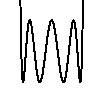
\includegraphics[height=1.75cm]{./../../common/images/Tcheb_008.pdf}
        \end{tabular}    
        &
        \begin{tabular}{c}
          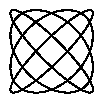
\includegraphics[height=1.75cm]{./../../common/images/Tcheb_2d_008.pdf}
        \end{tabular}    
      \end{tabular}
    \end{center}
    \vspace{-0.3cm}
Veien fra disse bildene til flatefasongene i det interaktive bildet, er ikke lang.


	S. V. \ Chmutov fant disse ligningene tidlig på 80-tallet. 
    På den tiden utgjorde de verdensrekorden for nesten alle grader $\mu(d)$ altså for det maksimale antallet singulariteter som en flate av grad $d$ kan ha.
    
	På 90-tallet forbedret Chmutov sin egen rekord, og i 2005 tilpasset 
	S.~Breske, O.~Labs og D.~van~Straten denne konstruksjonen slik at den også gjaldt 
	for reelle flater med bare reelle singulariteter.
\end{surferPage}
